\documentclass[14pt]{extreport}

\usepackage{geometry}
\geometry{a4paper,
          total={165mm,257mm},
          left=30mm,
          top=20mm,
         }

\usepackage[utf8]{inputenc}
\usepackage[T1]{fontenc}
\usepackage[english]{babel}
\usepackage{csquotes}

\usepackage[
    backend = biber,
    style = numeric,
]{biblatex}

\addbibresource{Refs.bib}

\usepackage{graphicx}
\graphicspath{ {./images/} }

\usepackage[table,xcdraw]{xcolor}

\usepackage{cmap}

\usepackage{hyperref}
\hypersetup{
    colorlinks=true,
    linkcolor=blue,
    filecolor=blue,
    urlcolor=blue,
    citecolor=blue,
    pdftitle={Titanic dataset analysis},
    pdfpagemode=FullScreen
}
\urlstyle{same}


\title{Titanic dataset analysis}
\author{Bogachev Aleksei}
\date{\today}


\begin{document}

    \maketitle

    \begin{abstract}
        Data analysis and models for the legendary machine learning
        competition on \href{https://www.kaggle.com/c/titanic}{Kaggle}.
    \end{abstract}

    \tableofcontents

    \chapter{Introduction}
Perhaps, the sinking of the RMS Titanic is the most infamous shipwreck 
in history. According to the 
\href{https://en.wikipedia.org/wiki/Titanic}{Wikipedia}, 
the RMS Titanic was the largest ocean liner in service at the time. It
had advanced safety features, such as watertight compartments and 
remotely activated watertight doors. The ship was widely considered 
"unsinkable". However, the Titanic sank in the early morning of 15 April
1912 in the North Atalntic Ocean during her maiden voyage from 
Southampton to New York City. There were an estimated 2224 people on
board when the ship collided with an iceberg
\cite{titanic-wikipedia},\cite{sinking-of-the-titanic-wikipedia}.

In accordance with existing practice, Titanic's lifeboat system was 
designed to ferry passengers to nearby rescue vessels, not to hold 
everyone on board simultaneously; therefore, with the ship sinking 
rapidly (the ship had sank in 2 hours and 40 minutes) and help still 
hours away, there was no safe refuge for many of the passengers and 
crew with only 20 lifeboats. Poor management of the evacuation meant 
many boats were launched before they were completely full 
\cite{sinking-of-the-titanic-wikipedia}.

The shipwreck resulted in the deaths of more than 1500 people, makng it 
one of the deadliest in history \cite{sinking-of-the-titanic-wikipedia}.

Without a doubt, there was an element of luck involved in surviving, but,
possibly, some groups of people were more likely to survive than others.
The \href{https://www.kaggle.com/c/titanic}{Titanic ML competition on 
Kaggle} offers participants to predict which of the passengers survived 
the shipwreck using passenger data\cite{titanic-ml-competition}.

In this report I'm going to describe my solution of the
\href{https://www.kaggle.com/c/titanic}{Titanic ML competition's} task.
My workflow will be based mostly on the
\href{https://github.com/ageron/handson-ml/blob/master/ml-project-checklist.md}
{"Machine Learning project checklist"} from the book \cite{hands_on_ml}.
I really appreciate this book and highly recommend reading it to anyone 
starting to learn about machine learning. 

Dozens of articles dedicated to this competition and hundreds of solutions 
of this task are available in the Internet. Therefore, I won't cite to 
all materials seen, but I'll try to give several useful refrences.

    \chapter{Task Description}
In this section the task is described according to 
\href{https://github.com/ageron/handson-ml/blob/master/ml-project-checklist.md}
{"Machine Learning project checklist"} \cite{hands_on_ml}.


\section{Goal}
To predict if a passanger survived the sinking of the Titanic or not.


\section{Crrent Solutions}
There are dosens of solutions available on 
\href{https://www.kaggle.com/c/titanic/discussion}{the discussion forum} 
and on the Internet.


\section{Frame the Problem}
\begin{itemize}
	\item Supervised learning
	\item Classification
	\item Binary classification (survived of not)
	\item Batch learning (no continuous flow of data and the dataset is 
	small)
\end{itemize}


\section{Performance metrics}
This competition evaluates the \textbf{percentage of correctly predicted
passengers} (accuracy).

There are also several useful metrics for evaluating the performance of 
a classification system:
\begin{itemize}
	\item precision,
	\item recall,
	\item $F_1$ score,
	\item precision/recall curve,
	\item ROC curve,
	\item ROC AUC score.
\end{itemize}


\section{Target performance}
The leaderboard of this competition contains almost 14000 entries. It's
available in the form of the csv-file. An excerpt from the leaderboard 
is presented in the table \ref{table:excert_from_leaderboard}.

\begin{table}[!ht]
	\centering
	\caption{Excerpt from the leaderboard}
	\begin{tabular}{|r|r|r|r|r|}
		\hline
		\textbf{TeamId} & \textbf{TeamName}       & \textbf{SubmissionDate} & \textbf{Score} \\ \hline
		6987444         & no name                 & 2022-08-23 18:16:28     & 1.0            \\ \hline
		720238          & rosh                    & 2022-06-26 10:58:42     & 1.0            \\ \hline
		8814675         & nikolai otvetchikov \#2 & 2022-06-26 13:59:39     & 1.0            \\ \hline
		8821160         & Vibhav Rathkanthiwar    & 2022-06-26 15:28:12     & 1.0            \\ \hline
		6590016         & Osman Altuntas          & 2022-07-24 15:40:15     & 1.0            \\ \hline
	\end{tabular}
	\label{table:excert_from_leaderboard}
\end{table}

The descriptive statistics is shown in the table
\ref{table:scores_statistics}.

\begin{table}[!ht]
	\centering
	\caption{Descriptive statistics of scores}
	\begin{tabular}{|r|r|}
	\hline
		\textbf{Statistics} & \textbf{Value}        \\ \hline
		count               & 13915.000000          \\ \hline
		mean                & 0.760751              \\ \hline
		std                 & 0.075145              \\ \hline
		min                 & 0.000000              \\ \hline
		25\%                & 0.765550              \\ \hline
		50\%                & 0.775110              \\ \hline
		75\%                & 0.777510              \\ \hline
		max                 & 1.000000              \\ \hline
	\end{tabular}
	\label{table:scores_statistics}
\end{table}

The median score is about 0.775, but less than 3\% of the solutions have 
a score above 0.8. Thus, \textbf{an accuracy score equal to or greater 
than 0.8 would be a very good result}. Figure \ref{pic:leaderboard_scores_ecdf}
shows ECDF of the scores in the leaderboard. In this figure, the red 
lines mark the score 0.8 and the corresponding proportion of solutions.

\begin{figure}[!ht]
	\centering
	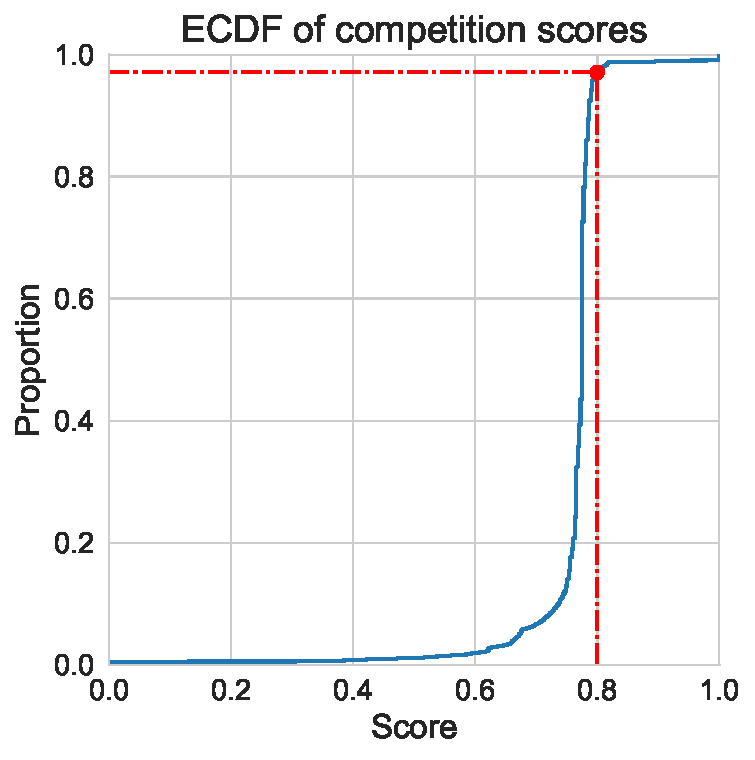
\includegraphics[width=0.5\textwidth]{leaderboard_scores_ecdf}
	\caption{Leaderboard Scores ECDF}
	\label{pic:leaderboard_scores_ecdf}
\end{figure}

There are several solutions with a score equal to 1.0. These solutions 
are marked with a red arrow in the figure \ref{pic:leaderboard_scores_kde}. 
Have authors reached perfection?

\begin{figure}[!ht]
	\centering
	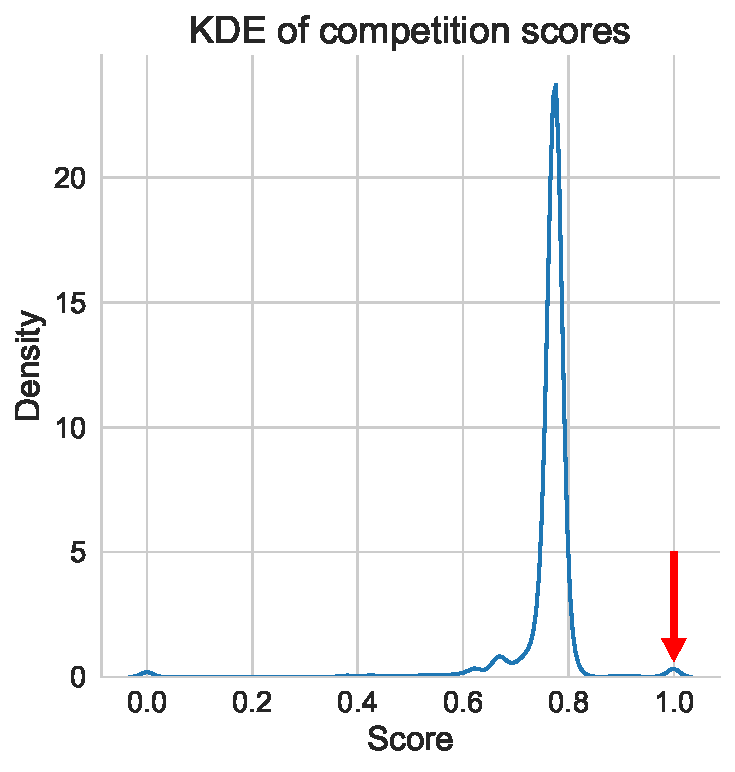
\includegraphics[width=0.5\textwidth]{leaderboard_scores_kde}
	\caption{Leaderboard Scores KDE}
	\label{pic:leaderboard_scores_kde}
\end{figure}

I guess, this solutions appears, because there is an exact solution on
\href{https://github.com/thisisjasonjafari/my-datascientise-handcode/raw/master/005-datavisualization/titanic.csv}
{GitHub}. Possibly it is the data extracted from 
\href{https://www.encyclopedia-titanica.org/titanic-survivors/}
{Encyclopedia Titanica}\cite{encyclopedia_titanica} or from
\href{https://www.openml.org/search?type=data&sort=runs&id=40945&status=active}
{OpenML}. Some authors in their notebooks honestly warn other users about 
the existence of such a possibility, for example, 
\href{https://www.kaggle.com/code/suzukifelipe/how-to-be-a-top-lb-explained-for-beginners/notebook?scriptVersionId=99817039}{this one}
\cite{perfection_explanation}.


\section{Data Dictionary}
\begin{enumerate}
	\item \textbf{PassengerId} -- Passenger ID.
	\item \textbf{Survived} -- Survival:
	\begin{itemize}
	    \item 0 = No, 
	    \item 1 = Yes.
	\end{itemize}
	\item \textbf{Pclass} -- Ticket class:
	\begin{itemize}	
	    \item 1 = 1st, 
	    \item 2 = 2nd, 
	    \item 3 = 3rd.
    \end{itemize}
	\item \textbf{Name} -- Passanger's name, for example, "Braund, 
	Mr. Owen Harris".
	\item \textbf{Sex} -- Gender:
	\begin{itemize}
	    \item male,
	    \item female.
	\end{itemize}
	\item \textbf{Age} -- Age in years, for example 38.0.
	\item \textbf{SibSp} -- Number of siblings or spouses aboard the Titanic.
	\item \textbf{Parch} -- Number of parents or children aboard the Titanic.
	\item \textbf{Ticket} -- Ticket number, for example, A/5 21171.
	\item \textbf{Fare} -- Passenger fare, for ecample, 71.2833.
	\item \textbf{Cabin} -- Cabin number, for example, C85.
	\item \textbf{Embarked} -- Port of Embarkation:
	\begin{itemize}
	    \item C = Cherbourg,
	    \item Q = Queenstown,
	    \item S = Southampton.
	\end{itemize}
\end{enumerate}


\subsection{Features}
PassengerId, Pclass, Name, Sex, Age, SibSp, Parch, Ticket, Fare, Cabin, 
\\Embarked


\subsection{Target}
Survived


\subsection{Variable Notes}
\begin{itemize}
	\item \textbf{pclass}: socio-economic status
		\begin{itemize}
		    \item 1st = Upper
		    \item 2nd = Middle
		    \item 3rd = Lower
		\end{itemize}
	\item \textbf{age}: Age is fractional if less than 1. If the age is 
	estimated, is it in the form of xx.5
	\item \textbf{sibsp} number of sibling/spouses aboard the Titanic
		\begin{itemize}
		    \item sibling = brother, sister, stepbrother, stepsister
		    \item spouse = husband, wife (mistresses and fiancés were 
		    ignored)
		\end{itemize}
	\item \textbf{parch} number of parents (mother, father)/children 
	(daughter, son, stepdauter, stepson) aboard the Titanic. Some 
	children travelled only with a nanny, therefore parch=0 for them.
\end{itemize}


\section{File Paths}
\begin{itemize}
	\item \textbf{training set}: \url{../datasets/train.csv}
	\item \textbf{test set}: \url{../datasets/test.csv}
	\item \textbf{example of a submission file}:
	\url{../datasets/gender_submission.csv}
\end{itemize}


\section{Assumptions}
Women were more likely to survive than men.
    
    \chapter{Preliminary Analysis}

\section{Shape of the dataset}
The dataset contains:
\begin{itemize}
	\item 891 rows, 
	\item 12 columns.
\end{itemize}


\section{First rows of the dataset} \label{section:first_rows}
An excerpt from the dataset is presented in the table
\ref{table:excerpt_from_dataset}.

\begin{table}[!ht]
	\centering
	\caption{Excerpt from the dataset}
	\resizebox{\textwidth}{!}{
	\begin{tabular}{|r|r|r|r|r|r|r|r|r|r|r|r|r|}
		\hline
		           & \textbf{PassengerId} & \textbf{Survived} & \textbf{Pclass} & \textbf{Name}                                     & \textbf{Sex} & \textbf{Age} & \textbf{SibSp} & \textbf{Parch} & \textbf{Ticket}  & \textbf{Fare} & \textbf{Cabin} & \textbf{Embarked} \\ \hline
		\textbf{0} & 1                    & 0                 & 3               & Braund, Mr. Owen Harris                           & male         & 22.0         & 1              & 0              & A/5 21171        & 7.2500        & NaN            & S                 \\ \hline
		\textbf{1} & 2                    & 1                 & 1               & Cumings, Mrs. John Bradley (Florence Briggs Th... & female       & 38.0         & 1              & 0              & PC 17599         & 71.2833       & C85            & C                 \\ \hline
		\textbf{2} & 3                    & 1                 & 3               & Heikkinen, Miss. Laina                            & female       & 26.0         & 0              & 0              & STON/O2. 3101282 & 7.9250        & NaN            & S                 \\ \hline
		\textbf{3} & 4                    & 1                 & 1               & Futrelle, Mrs. Jacques Heath (Lily May Peel)      & female       & 35.0         & 1              & 0              & 113803           & 53.1000       & C123           & S                 \\ \hline
		\textbf{4} & 5                    & 0                 & 3               & Allen, Mr. William Henry                          & male         & 35.0         & 0              & 0              & 373450           & 8.0500        & NaN            & S                 \\ \hline
	\end{tabular}}
	\label{table:excerpt_from_dataset}
\end{table}

The \textbf{"PassengerId"} feature is the ID of the passanger. It won't 
help in the analysis and will be dropped. Also, there are several missing 
values, and some values are categorical, for example, \textbf{"Pclass"}
and \textbf{"Sex"}.


\section{Data types and missing values}
Table \ref{table:dtypes} contains types of the data in each column and
numbers of non-null values. Table \ref{table:missing_values} contains 
numbers of missing values in each column.

\begin{table}[!ht]
	\centering
	\caption{Data types and non-null counts}
	\begin{tabular}{|l|l|l|l|}
		\hline
		\textbf{\#} & \textbf{Column} & \textbf{Non-Null Count} & \textbf{Dtype} \\ \hline
		\textbf{0}  & PassengerId     & 891 non-null            & int64          \\ \hline
		\textbf{1}  & Survived        & 891 non-null            & int64          \\ \hline
		\textbf{2}  & Pclass          & 891 non-null            & int64          \\ \hline
		\textbf{3}  & Name            & 891 non-null            & object         \\ \hline
		\textbf{4}  & Sex             & 891 non-null            & object         \\ \hline
		\textbf{5}  & Age             & 714 non-null            & float64        \\ \hline
		\textbf{6}  & SibSp           & 891 non-null            & int64          \\ \hline
		\textbf{7}  & Parch           & 891 non-null            & int64          \\ \hline
		\textbf{8}  & Ticket          & 891 non-null            & object         \\ \hline
		\textbf{9}  & Fare            & 891 non-null            & float64        \\ \hline
		\textbf{10} & Cabin           & 204 non-null            & object         \\ \hline
		\textbf{11} & Embarked        & 889 non-null            & object         \\ \hline
	\end{tabular}
	\label{table:dtypes}
\end{table}

\begin{table}[!ht]
	\centering
	\caption{Number of missing values in each column}
	\begin{tabular}{|l|l|l|}
		\hline
		\textbf{\#} & \textbf{Column}   & \textbf{Number of missing values} \\ \hline
		\textbf{0}  & PassengerId       & 0                                 \\ \hline
		\textbf{1}  & Survived          & 0                                 \\ \hline
		\textbf{2}  & Pclass            & 0                                 \\ \hline
		\textbf{3}  & Name              & 0                                 \\ \hline
		\textbf{4}  & Sex               & 0                                 \\ \hline
		\textbf{5}  & \textbf{Age}      & \textbf{177}                      \\ \hline
		\textbf{6}  & SibSp             & 0                                 \\ \hline
		\textbf{7}  & Parch             & 0                                 \\ \hline
		\textbf{8}  & Ticket            & 0                                 \\ \hline
		\textbf{9}  & Fare              & 0                                 \\ \hline
		\textbf{10} & \textbf{Cabin}    & \textbf{687}                      \\ \hline
		\textbf{11} & \textbf{Embarked} & \textbf{2}                        \\ \hline
	\end{tabular}
	\label{table:missing_values}
\end{table}


\pagebreak
\section{Number of unique values}
Table \ref{table:unique_values} contains numbers of unique values in 
each column.

\begin{table}[!ht]
	\centering
	\caption{Number of unique values in each column}
	\resizebox{\textwidth}{!}{
	\begin{tabular}{|
	>{\columncolor[HTML]{EFEFEF}}l |l|
	>{\columncolor[HTML]{EFEFEF}}l |l|}
		\hline
		\textbf{Column} & \textbf{Number of unique values} & \textbf{Column} & \textbf{Number of unique values} \\ \hline
		Name            & 891                              & Survived        & 2                                \\ \hline
		Sex             & 2                                & Pclass          & 3                                \\ \hline
		Ticket          & 681                              & Age             & 88                               \\ \hline
		Cabin           & 147                              & SibSp           & 7                                \\ \hline
		Embarked        & 3                                & Parch           & 7                                \\ \hline
		PassengerId     & 891                              & Fare            & 248                              \\ \hline
	\end{tabular}}
	\label{table:unique_values}
\end{table}

There are high-cardinality features with \textit{object} dtype:
\begin{itemize}
	\item Name
	\item Ticket
	\item Cabin
	\item PassengerId
\end{itemize}
This features, possibly, will need special preprocessing. Earlier, I
noticed that the \textbf{"PassengerId"} feature is the ID of the
passanger. It won't help in the analysis and will be dropped. 

Features \textbf{"Age"} and \textbf{"Fare"} are continuous.


\section{Summary statistics}
In this section, summary statistics for numerical and non-numerical 
attributes are presented in tables \ref{table:numerical_variable_description}
and \ref{table:categorical_variable_description} respectively.

\begin{table}[!ht]
	\centering
	\caption{Summary statistics for numerical attributes}
	\resizebox{\textwidth}{!}{
	\begin{tabular}{|r|r|r|r|r|r|r|r|}
		\hline
		               & \textbf{PassengerId} & \textbf{Survived} & \textbf{Pclass} & \textbf{Age} & \textbf{SibSp} & \textbf{Parch} & \textbf{Fare} \\ \hline
		\textbf{count} & 891.000000           & 891.000000        & 891.000000      & 714.000000   & 891.000000     & 891.000000     & 891.000000    \\ \hline
		\textbf{mean}  & 446.000000           & 0.383838          & 2.308642        & 29.699118    & 0.523008       & 0.381594       & 32.204208     \\ \hline
		\textbf{std}   & 257.353842           & 0.486592          & 0.836071        & 14.526497    & 1.102743       & 0.806057       & 49.693429     \\ \hline
		\textbf{min}   & 1.000000             & 0.000000          & 1.000000        & 0.420000     & 0.000000       & 0.000000       & 0.000000      \\ \hline
		\textbf{25\%}  & 223.500000           & 0.000000          & 2.000000        & 20.125000    & 0.000000       & 0.000000       & 7.910400      \\ \hline
		\textbf{50\%}  & 446.000000           & 0.000000          & 3.000000        & 28.000000    & 0.000000       & 0.000000       & 14.454200     \\ \hline
		\textbf{75\%}  & 668.500000           & 1.000000          & 3.000000        & 38.000000    & 1.000000       & 0.000000       & 31.000000     \\ \hline
		\textbf{max}   & 891.000000           & 1.000000          & 3.000000        & 80.000000    & 8.000000       & 6.000000       & 512.329200    \\ \hline
	\end{tabular}}
	\label{table:numerical_variable_description}
\end{table}

\begin{table}[!ht]
	\centering
	\caption{Summary statistics for non-numerical attributes}
	\begin{tabular}{|r|r|r|r|r|r|}
		\hline
		                & \textbf{Name}           & \textbf{Sex} & \textbf{Ticket} & \textbf{Cabin} & \textbf{Embarked} \\ \hline
		\textbf{count}  & 891                     & 891          & 891             & 204            & 889               \\ \hline
		\textbf{unique} & 891                     & 2            & 681             & 147            & 3                 \\ \hline
		\textbf{top}    & Braund, Mr. Owen Harris & male         & 347082          & B96 B98        & S                 \\ \hline
		\textbf{freq}   & 1                       & 577          & 7               & 4              & 644               \\ \hline
	\end{tabular}
	\label{table:categorical_variable_description}
\end{table}


\section{Proportion of target values}

Let's check if one class of target values is more frequent than another.

Figure \ref{number_of_survivors} illustrates these numbers. There are 342 
(38.38\%) survived passengers and 549 (61.62\%) drowned passengers in the 
dataset, so the dataset is a bit skewed. Therefore, the accuracy may not be 
sufficient to assess the performance of classifiers.

\begin{figure}[!ht]
	\centering
	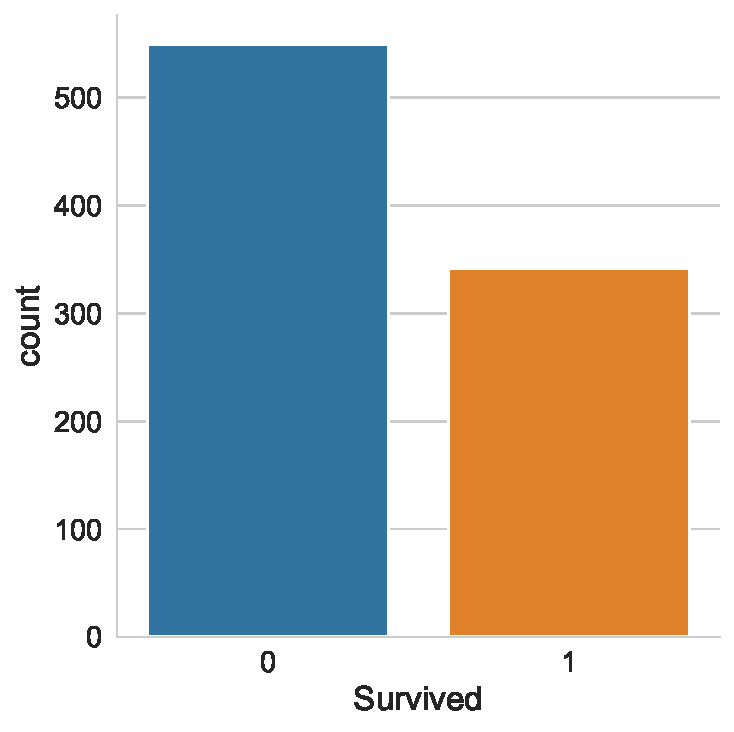
\includegraphics[width=0.5\textwidth]{number_of_survivors}
	\caption{Number of survived and drowned passangers in whole dataset}
	\label{number_of_survivors}
\end{figure}

    \chapter{Sample a Test Set} \label{chapter:sample_test_set}
The test set will be used to evaluate performance of a very final model
and forecast the score in the competitions leaderboard. It may seems like
it's to early to create a test set, but I'll do it to prevent data snooping.

I'm going to do stratified sampling with scikit-learn's \texttt{StraifiedShuffleSplit}
to maintain equal ratio of men and women in the train set and the test set.
Women seem to have had a better chance of surviving due to the "women and
children first" protocol for loading lifeboats.

Next, let's check the proportion of women among all survivors (figure
\ref{proportion_of_survived_women}), and check the proportion of survived
women in each \textbf{"Pclass"} (figure 
\ref{proportion_of_survived_women_among_pclasses}).

\begin{figure}[!ht]
	\centering
	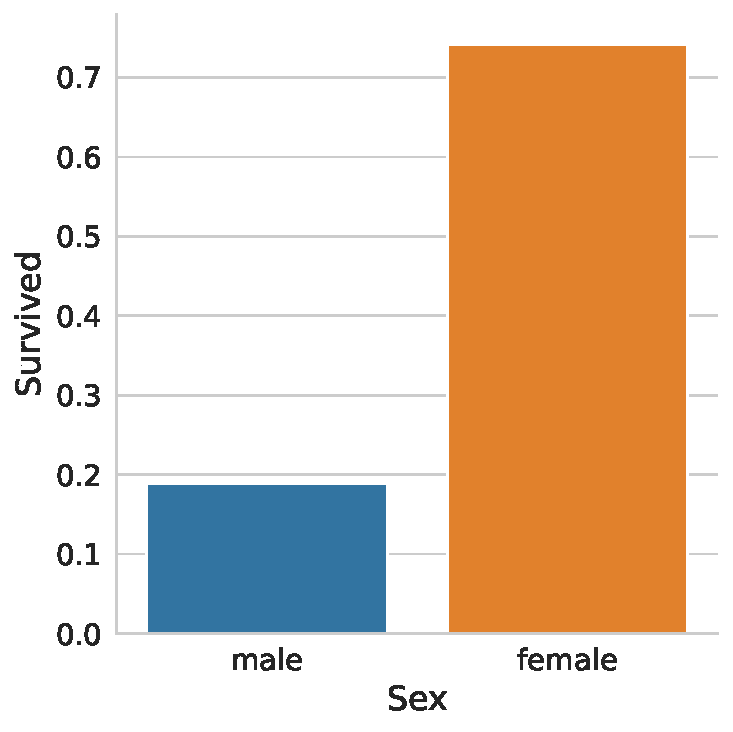
\includegraphics[width=0.5\textwidth]{proportion_of_survived_women}
	\caption{Proportions of survived men and women}
	\label{proportion_of_survived_women}
\end{figure}

\begin{figure}[!ht]
	\centering
	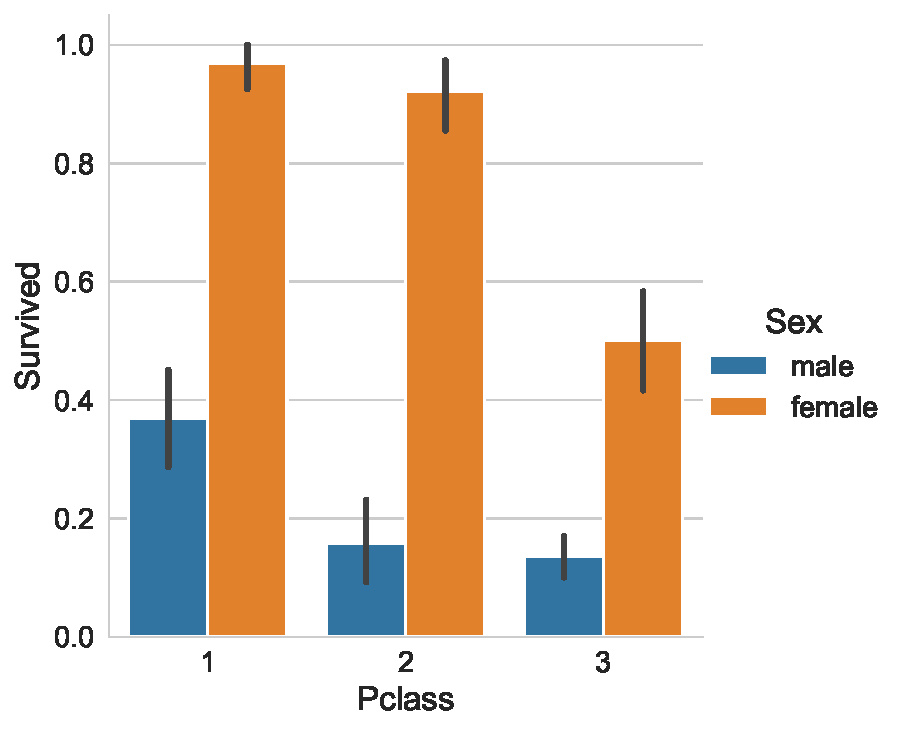
\includegraphics[width=0.5\textwidth]{proportion_of_survived_women_among_pclasses}
	\caption{Proporotion of survived women and men in each \textbf{"Pclass"}}
	\label{proportion_of_survived_women_among_pclasses}
\end{figure}

Figures \ref{proportion_of_survived_women} and 
\ref{proportion_of_survived_women_among_pclasses} show that in the entire 
dataset and in each \textbf{"Pclass"}, there are more female survivors 
than males. Thus it is reasonable to do stratification based on the
passenger's gender. I will use 80\% of the data for training and hold 
out 20\% for testing, refer to the Jupyter Notebook for details.

    \printbibliography[heading=bibintoc, 
                       title={References}]

\end{document}